\documentclass[letterpaper, 10pt, conference]{ieeeconf}
% IEEE RA-L submission — PaperCept template (ieeeconf), A4 per RA-L rules.
% Limit: 6 pages + max 2 extra pages (at charge) = 8 pages hard cap.

\IEEEoverridecommandlockouts
\overrideIEEEmargins
\addtolength{\topmargin}{9pt}
\addtolength{\textheight}{6pt}

\usepackage{graphicx}
\usepackage{amsmath}
\usepackage{booktabs}
\usepackage{array}
\usepackage[caption=false,font=footnotesize]{subfig}
\usepackage{multirow}

\title{\LARGE \bf
Graded Fault Response for Autonomous Driving via Continuous Sensor Health
Monitoring and Risk/Capability-Aware MRM Supervision}

% RA-L initial submission is double-anonymous: swap in the anonymous block
% and comment out the named block before submitting.
%\author{Anonymous Submission\thanks{Author information omitted for
%double-anonymous review.}}
\author{Tae Wook Eum, Jun Hyeon Choi, Ye Chan An, Jin Ho Kim, and Tae Yong Kuc%
\thanks{This work was supported by the BK21 FOUR Project. Corresponding author: Tae Yong Kuc.}%
\thanks{The authors are with the Department of Electrical and Computer
Engineering, Sungkyunkwan University, Suwon 16419, Republic of Korea
(e-mail: utsi09@g.skku.edu, choijunhyeon@g.skku.edu, ycan@g.skku.edu,
wasabi9812@naver.com, tykuc@skku.edu).}%
}

\begin{document}

\maketitle
\thispagestyle{empty}
\pagestyle{empty}

\begin{abstract}
Sensor-fault handling in automated driving stacks largely reduces to an
immediate in-lane stop, while undetected degradation lets the vehicle keep
driving with impaired perception. We propose a graded fault-response layer
added onto an unmodified Autoware stack: (i) a behavior-tree monitor
estimating per-sensor health as continuous scores (freshness, quality,
physics) composed into capability scores, and (ii) an MRM
supervisor selecting between shoulder/parking evacuation and deferral to
the stock stop by fault type, severity, and remaining capability, with a
conservative 3.0~m/s cap on evacuation movement. Across 1{,}862 valid
closed-loop CARLA cases, detection reached 96--100\% in every condition
except one tolerated by design, with zero false activations, and
degraded-state exposure fell from 238--275~m to 11--58~m. Verdicts rest on a dual
scheme---an ego collision ledger and a pedestrian physics oracle---built
after finding silent collision sensors. A
pre-registered dose-response experiment (3 caps $\times$ 4 distances
$\times$ 10 seeds) shows the cap causally moves the avoid/collide boundary
inward (8~m: discordant pairs 10:0, exact McNemar $p=0.002$); encounters in
the post-detection deceleration transient remain at risk.
\end{abstract}

\section{INTRODUCTION}

Automated driving systems at SAE Level~4 and above cannot presuppose
driver intervention: upon a fault they must reach a minimal risk condition
(MRC) via a minimal risk maneuver (MRM) on their own. ISO~26262 requires
detection and response within the fault-tolerant time interval (FTTI), and
SOTIF (ISO~21448) requires managing hazards from sensor performance
limitations~\cite{iso26262,iso21448,j3016}. In the open-source stack
Autoware, the default MRMs are in-lane stops (comfortable/emergency), and its
stock diagnostics primarily target communication- and hardware-level
anomalies such as topic silence and timeouts~\cite{autoware}. In the version
and execution configuration evaluated in this study (Autoware 0.39.0),
degradation faults whose values stay within valid ranges left driving to
continue without intervention, and no supervisory layer existed that
evaluates fault type and degree together with remaining maneuvering
capability, selects between evacuation and stopping, and limits evacuation
speed to match the fault state. That supervisory layer---not the shoulder
maneuver itself---is the contribution of this work; the observation is
version-specific, not a claim about Autoware in general.

An in-lane stop is simple and immediate, but the stopped vehicle blocks
traffic and creates secondary-collision exposure until the lane clears. Conversely, driving on with an undetected fault extends the distance
exposed to hazards under degraded perception---in our unmonitored
observations (one run per fault type) the stock stack completed 238--275~m
of route with faults injected. The design space of fault response has three axes: \emph{whether to stop
now, how far to move, and---if moving---how fast}.

Automating human-driver-like shoulder evacuation requires
(i)~distinguishing faults mild enough to permit moving from faults
requiring an immediate stop; (ii)~a continuous estimate of fault type and
degree (a binary normal/faulty state is insufficient); and (iii)~managing
the risk of moving itself in a degraded state---the stopping distance
against a dart-out. We implement these as a continuous health score,
risk/capability-based state transitions, and a conservative speed cap.

Finally, simulation-based safety claims stand only on the reliability of
the collision verdict itself: we empirically uncovered a simulator
collision-sensor configuration that remained silent, and built a dual
adjudication scheme---a real-time ego collision-sensor ledger and a
pedestrian physics oracle---on which every safety conclusion rests.

\textbf{Contributions.}
(1)~A behavior-tree monitor that scores per-sensor freshness, quality, and
physical consistency independently and composes them over eight spatial
sectors into perception/localization capability scores, published as
continuous health.
(2)~A risk/capability-aware MRM supervisor that selects between
shoulder/parking evacuation (\texttt{MRM\_MOVE}) and deferral to the stock
stop (\texttt{MRM\_DEFER}) by health-score bands, chooses the refuge by a
cost function over degraded-state exposure time, traffic-light
observability, and sector deficits, and imposes a fixed 3.0~m/s cap
(below the model-derived bound $\approx$3.9~m/s) on evacuation movement.
(3)~A dual collision-adjudication methodology (ego RAW-HIT ledger +
pedestrian physics oracle) with a catalogue of verdict pitfalls in runner
exit labels and official infraction records.
(4)~Validation totalling 1{,}862 valid closed-loop cases, including a
pre-registered dose-response experiment verifying the causal cap effect on
settled encounters, and transient-vs-settled observations locating
residual evacuation risk in the post-detection transient.

The novelty is not in the individual techniques (CUSUM, residual monitoring,
noisy-OR fusion, stopping-distance model---each known), but in the
integrated supervisory layer spanning detection through selection and speed,
and in the closed-loop demonstration whose verdict reliability is secured at
the methodological level.

\section{RELATED WORK}

\textbf{Standards and fault models.} Functional-safety and SOTIF
frameworks \cite{iso26262,iso21448,j3016} require runtime monitoring and
responses to degradation; ISO~23793-1~\cite{iso23793} taxonomizes MRM
types but covers only in-lane stops, and industrial
ISO~3691-4~\cite{iso3691} prescribes ``limited speed for limited
capability,'' which we transfer to on-road MRM. None provides a way to
continuously estimate fault kind and degree and select response and speed.
Classical FDI---residual generation/decision~\cite{isermann} and
sequential change detection (our LiDAR channel borrows CUSUM)---ends at
detection. Our fault models follow measured LiDAR soiling~\cite{trierweiler},
rain scattering~\cite{goodin}, and GNSS correlated bias~\cite{langel}.

\textbf{Fallback and MRM planning.} Fail-safe trajectory
planning~\cite{pek} maintains stop trajectories and online verification but
takes the fault assessment and response choice as given. Reschka and Maurer~\cite{reschka2015safe} noted that an in-lane stop is
not always a safe state---the concern we start from. Closest to us, Xue
\emph{et al.}~\cite{xue2018} presuppose a forward-sensor fault and plan
safe-zone stops under MPC constraints, and Tang \emph{et al.}~\cite{tang}
adaptively select MRM behaviors under multiple sensor faults via HAZOP
risk analysis with TTC/THW evaluation. They differ in that
(i)~the fault state is presupposed rather than estimated online;
(ii)~selection uses surrounding-traffic TTC/THW, whereas we combine risk
grace time with remaining perception/localization capability and limit the
evacuation speed itself; (iii)~validation checks representative scenarios,
whereas we verify 1{,}862 cases on a real stack with methodologically
secured encounter verdicts. Capability-based self-monitoring models abilities for online
decisions~\cite{reschka2015ability}; our sector composition couples
capability scores directly to MRM selection and the cap (behavior trees as the
implementation structure).

\textbf{Simulation-based evaluation.} CARLA~\cite{carla} hosts
fault-injection studies that inject faults to \emph{find}
vulnerabilities---the opposite direction from ours, where the stack itself
detects, grades, and responds. Our infrastructure builds on
AWCL~\cite{awcl}, the TUM Autoware--CARLA coupling. We found no prior
report addressing simulated collision-verdict reliability at the
methodology level.

\section{PROPOSED SYSTEM}

\begin{figure*}[t]
\centering
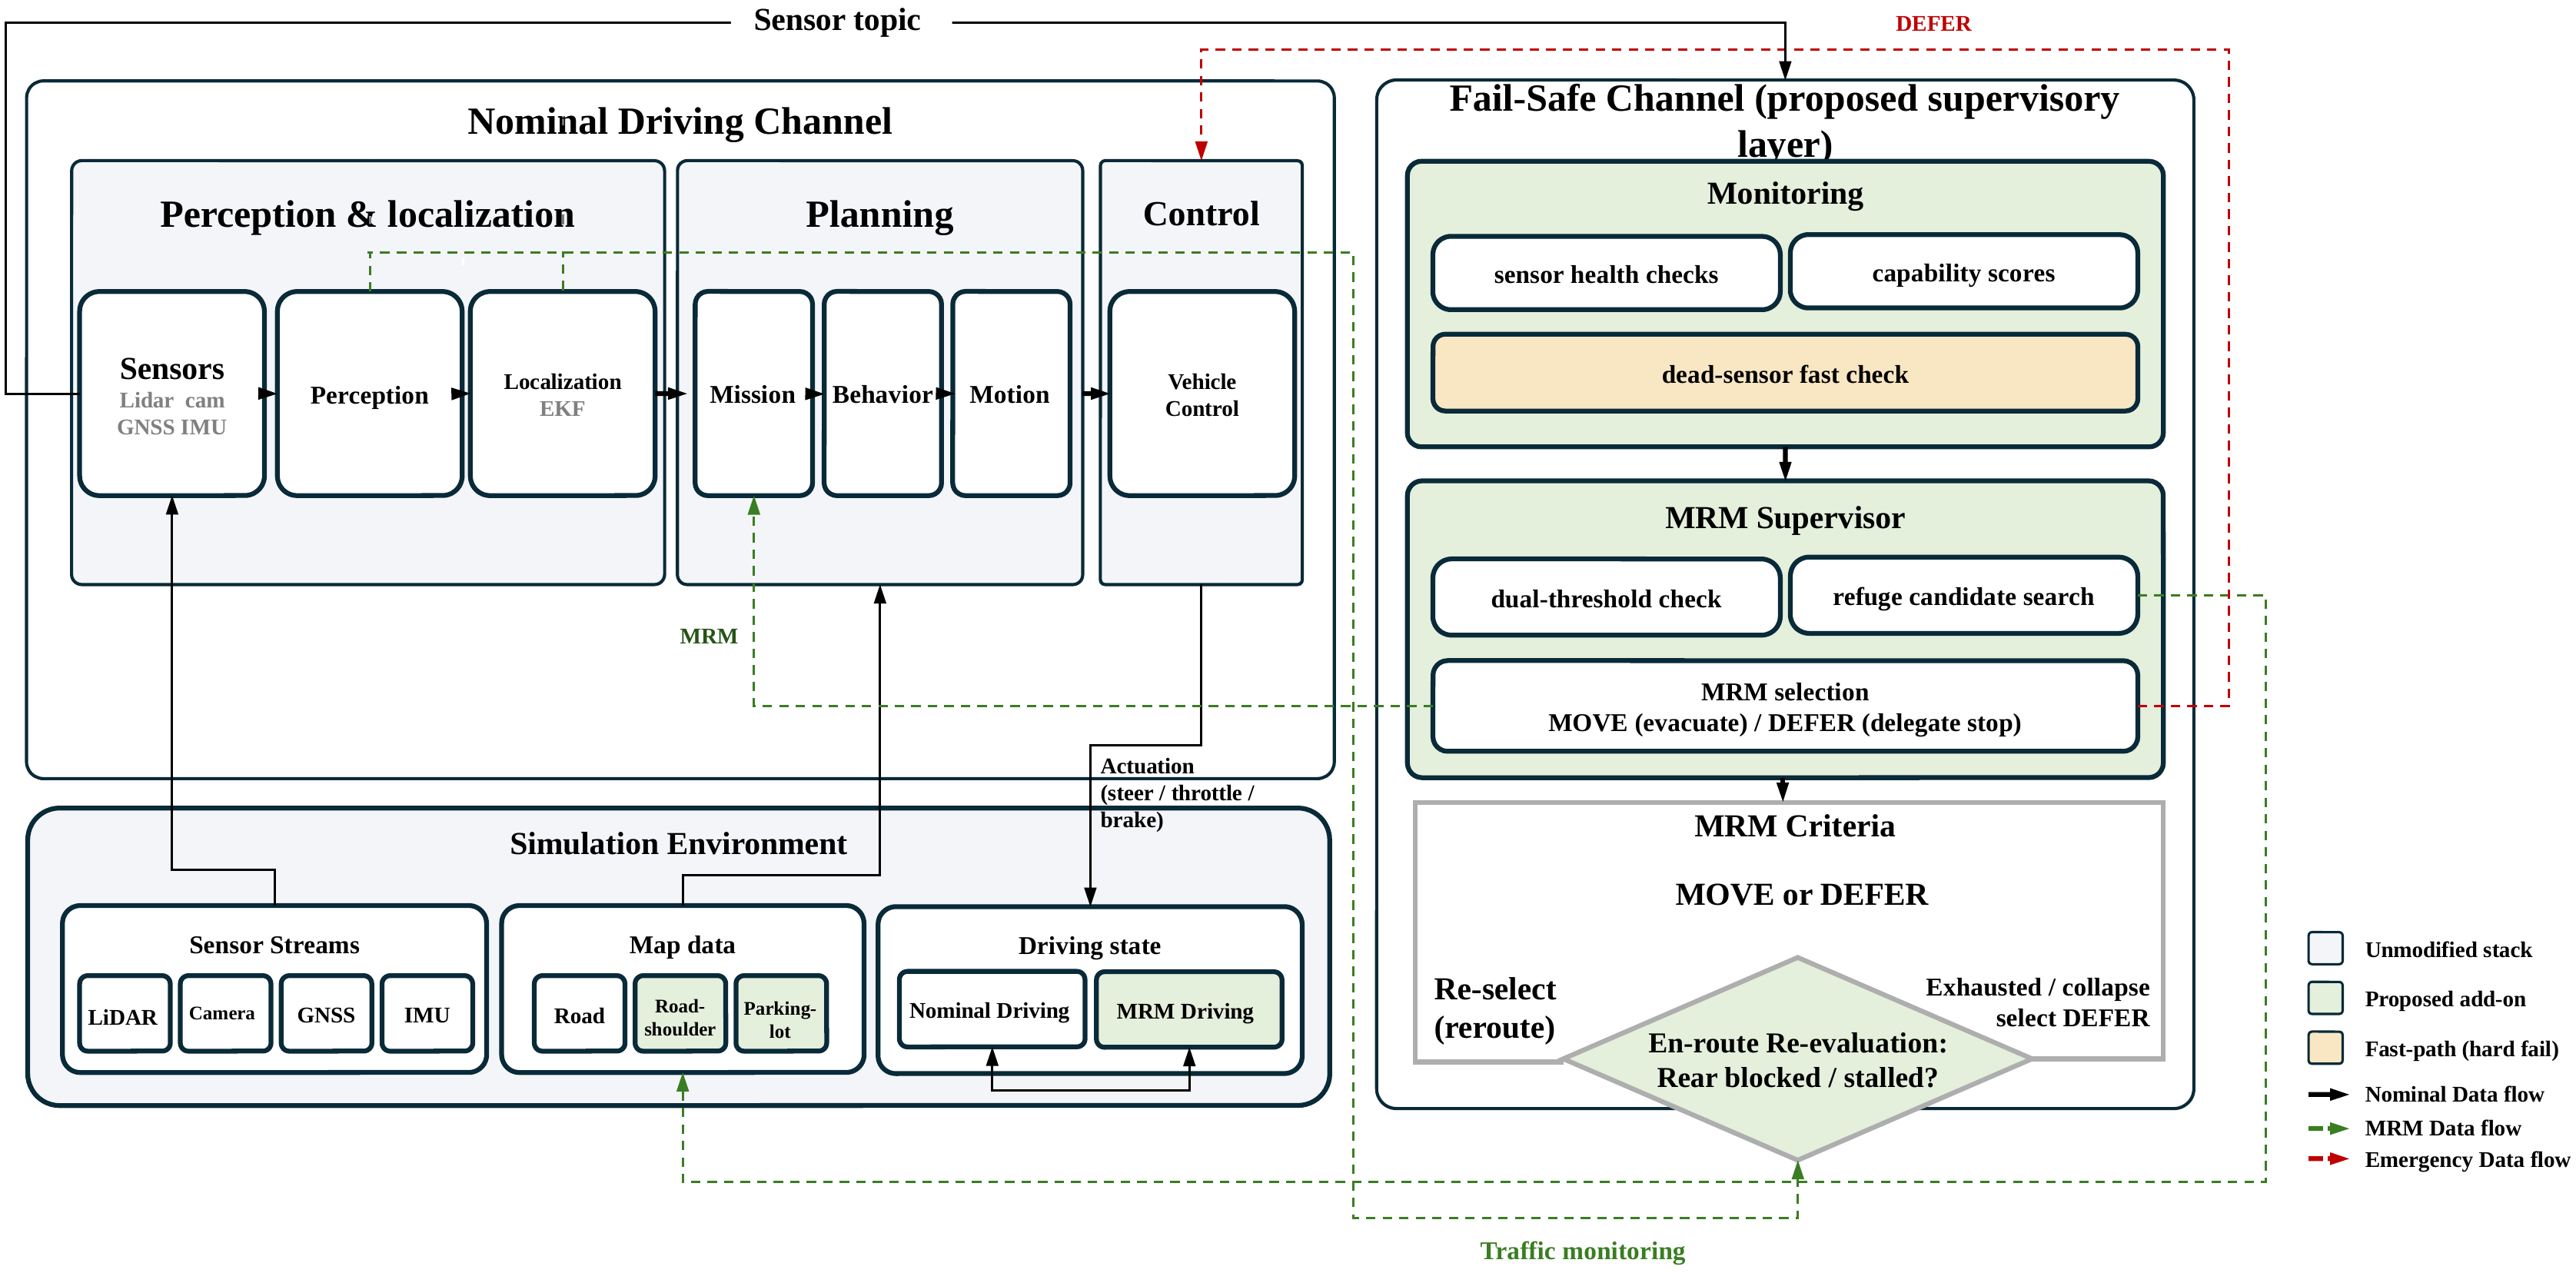
\includegraphics[width=0.68\textwidth]{figs/fig2b_dualchannel.png}
\caption{Dual-channel structure. Left: the nominal driving channel of
unmodified Autoware; right: the proposed supervisory layer---monitoring
subscribes read-only to sensor topics and produces health/capability
scores; the decision stage selects MOVE (evacuate: reroute with a speed
cap) or DEFER (inject a diagnostic ERROR to trigger the stock stop),
re-evaluating rear occupancy and stalls en route. Bottom: the CARLA closed
loop; refuge search draws on annotated map data.}
\label{fig:arch}
\vspace{-2mm}
\end{figure*}

\subsection{Architecture}
The system consists of two independent add-on nodes
(Fig.~\ref{fig:arch}). The monitoring module inspects each sensor at 10~Hz
on a behavior-tree basis, computing a per-sensor health score in $[0,1]$
from three detector families: timeout (freshness), quality (noise, valid
ratio), and physics (residual, bias). The MRM supervisor subscribes to the
scores and runs a state machine: for evacuation it changes the route via
the Autoware AD API and imposes a speed cap on the planning layer; for
deferral it triggers the stock \texttt{mrm\_handler} stop through the
diagnostic graph. Maneuver execution is delegated to the stock stack; the
main stack is not modified. Reception accumulates at native sensor rates;
evaluation runs at 10~Hz (AUTOSAR watchdog-style periodic supervision).

\subsection{Sensor Scoring}
\emph{Freshness.} For elapsed time $\mathrm{age}(t)$ since last
reception, $s_{\mathrm{fresh}}=\max(0,\,1-\mathrm{age}/\tau_{\mathrm{detect}})$
decays linearly---the score can cross the downstream band boundary before
the budget is exhausted, enabling early transition under silence; a
$k$-miss rule penalizes early on $3\times$ the median reception interval.

\emph{Quality.} For LiDAR, a noise level
$\hat{\sigma}=\overline{|\Delta r|}\cdot\sqrt{\pi}/2$ (neighboring-point
range differences, $|\Delta r|<1$~m) is referenced to a boot-time baseline
that refuses to track abrupt rises (the fault cannot become its own
baseline); the score is $\exp(-\max(0,\hat{\sigma}-\mathrm{base})/0.1)$
times a valid-point-ratio score, with a parallel CUSUM test so detection
delay is inversely proportional to fault magnitude. Camera quality applies
the same structure on inter-frame pixel differences (no cumulative test:
they rise with scene motion). Sparsification is caught by the valid-ratio
channel, clutter by the range-discontinuity channel.

\emph{Localization (three channels).} (a)~a residual channel on the
GNSS--EKF distance (sensitive to noise and correlated bias); (b)~a bias
channel comparing 3-s means of IMU and EKF yaw rates (normal turning
cancels; gyro bias remains on the IMU side); (c)~a silence channel decaying
the score when GNSS input stops $\ge$1~s while driving---covering the
residual channel's blind spot of freezing at the last value.

\subsection{Sector and Capability Synthesis}
Sensor scores map to eight directional sectors by mounting direction and
field of view and fuse as $s_{\mathrm{sector}}=1-\prod_i(1-s_i)$;
perception capability is a front-weighted sector sum combined with
traffic-light observability at $0.6{:}0.4$; system health is
$\min(\mathrm{perception},\,\mathrm{cap_{loc}})$---the weakest link.

\subsection{Risk-Coupled Detection Budget}
The freshness decay constant is coupled to driving risk:
$\tau_{\mathrm{detect}}(t)=\min(\tau_{\mathrm{fresh}},\,
\mathrm{TTC}_{\mathrm{cons}}(t))$, where
$\mathrm{TTC}_{\mathrm{cons}}$ is the minimum of nearest-obstacle TTC and
path-crossing time with a fail-conservative hold when the TTC source itself
is unhealthy. The design intent is
$T_{\mathrm{detect}}+T_{\mathrm{response}}+T_{\mathrm{margin}}\le
T_{\mathrm{hazard}}$; the implementation is a risk-adaptive heuristic
approximation, not a formal guarantee (explicit FRTI/margin reservation is
future work). For degradation faults the requirement is a severity curve
$T_{\mathrm{detect}}(\sigma)\le T_{\mathrm{hazard}}(\sigma)$.

\subsection{MRM Supervisor}
Dual thresholds on health (upper~0.7, lower~0.3) span three bands:
NORMAL, evacuation (\texttt{MRM\_MOVE}), and deferral
(\texttt{MRM\_DEFER}, on floor entry or localization-confidence collapse);
decay constants leave a wide insensitive gap between faulted and normal
scores, so behavior follows the band structure, not precise threshold
placement. Timing splits by evidence type: degradation faults are statistical
evidence requiring sustained confirmation (1.0~s band entry; 2.0~s at the
floor since deferral is terminal; a 5.0~s recovery grace, unchanged under a
0.5--5.0~s sensitivity sweep), whereas hard fails (silence past the 850~ms
freshness deadline) already carry accumulated evidence: confirmations are
skipped and unrecoverable conditions defer immediately. Selection is not frozen while moving: sustained rear occupancy demotes
reversing parking candidates to a shoulder stop, stalls get bounded
retries, and exhaustion or health collapse falls back to DEFER.

Refuge selection minimizes
\begin{multline}
J(c)=w_t\,\eta(c)+w_{tl}\,n_{tl}(c)\,g(tl)\\
 + w_{sec}\!\sum(1-s_{\mathrm{req}})+w_{loc}\,\eta(c)(1-\mathrm{loc}),
\end{multline}
where $\eta(c)$ is degraded-state exposure time (route time + expected
signal waits)---risk accumulates per unit \emph{time}, not distance. Route
times and traffic-light counts are computed on an in-house road-network
graph parsed directly from the lanelet2 map, keeping the decision layer
outside the influence of main-stack faults. The key safeguard is the
traffic-light observability gate: a candidate whose route passes signals no
healthy camera can read is excluded with $J=\infty$. Shoulder/parking
candidates are manually annotated map attributes (16 shoulders, 4 lots on
the test map).

\subsection{Conservative Low-Speed MRM Movement (Speed Cap)}
Evacuation is movement under degraded perception, so stopping capability
against a dart-out dominates. With reaction time $\tau$ and deceleration
$a$, stopping from speed $v$ requires
\begin{equation}
d_{\mathrm{safe}}(v)=v\tau+\frac{v^2}{2a}+d_{\mathrm{margin}}\le
D_{\mathrm{avail}}.
\label{eq:stop}
\end{equation}
Here $\tau\!\approx\!1.5$~s, $a\!\approx\!3.5$~m/s$^2$ are nominal
lumped values calibrated to the measured ladder boundary---a design
approximation, not a predictive safety model. On entering \texttt{MRM\_MOVE} the supervisor imposes a fixed 3.0~m/s
cap, chosen inside the band between the model-inverted cap that still
stops within an 8~m dart-out ($\approx$3.9~m/s) and the requirement that
evacuation-completion time stay bounded; no in-band optimization is
claimed. The cap feeds Autoware's velocity-limit arbiter, and delivery is
verified by \emph{measured vehicle speed}, not publish records---an
interface mismatch that silently dropped the cap in earlier runs was
caught exactly this way and corrected (Sec.~\ref{sec:dose}).

\section{EXPERIMENTAL SETUP}

\subsection{Environment and Campaign Matrix}
The closed loop couples CARLA~0.9.16 with Autoware~0.39.0 over the AWCL
bridge~\cite{awcl} on Town07 (annotated custom vector map; speed limit
15~km/h); the simulator is fully restarted for every case. A case is \{method, fault, severity, traffic, repetition, injection
time\}; methods are \emph{ours}, \emph{baseline} (identical detection,
deferral to the stock stop---isolating response strategy from detection),
and \emph{mrm-off} (passive scoring only). The main campaign is fault~$\times$ severity~$\times$ traffic density
(none/defensive/aggressive)~$\times$ method with 1{,}131 valid cases (39
short of plan, all in high-severity LiDAR clutter); a navigation-extension
matrix adds four navigation faults (611 valid), and encounter experiments
complete the 1{,}862 total.
The fault model injects inside the agent's sensor pipeline: camera
death/noise (cf/cn), LiDAR death/sparsification/clutter (lf/lso/lcl,
physical models~\cite{trierweiler,goodin}), GNSS noise/correlated
bias/outage (gn/gb/gf~\cite{langel}), and IMU noise/bias/drift (imn/imb/imd),
with severities low/mid/high where applicable; injection times and fault
waveforms are seed-fixed for pairing. Fig.~\ref{fig:faults} illustrates the
sensor-level effect of each injection.

\begin{figure*}[t]
\centering
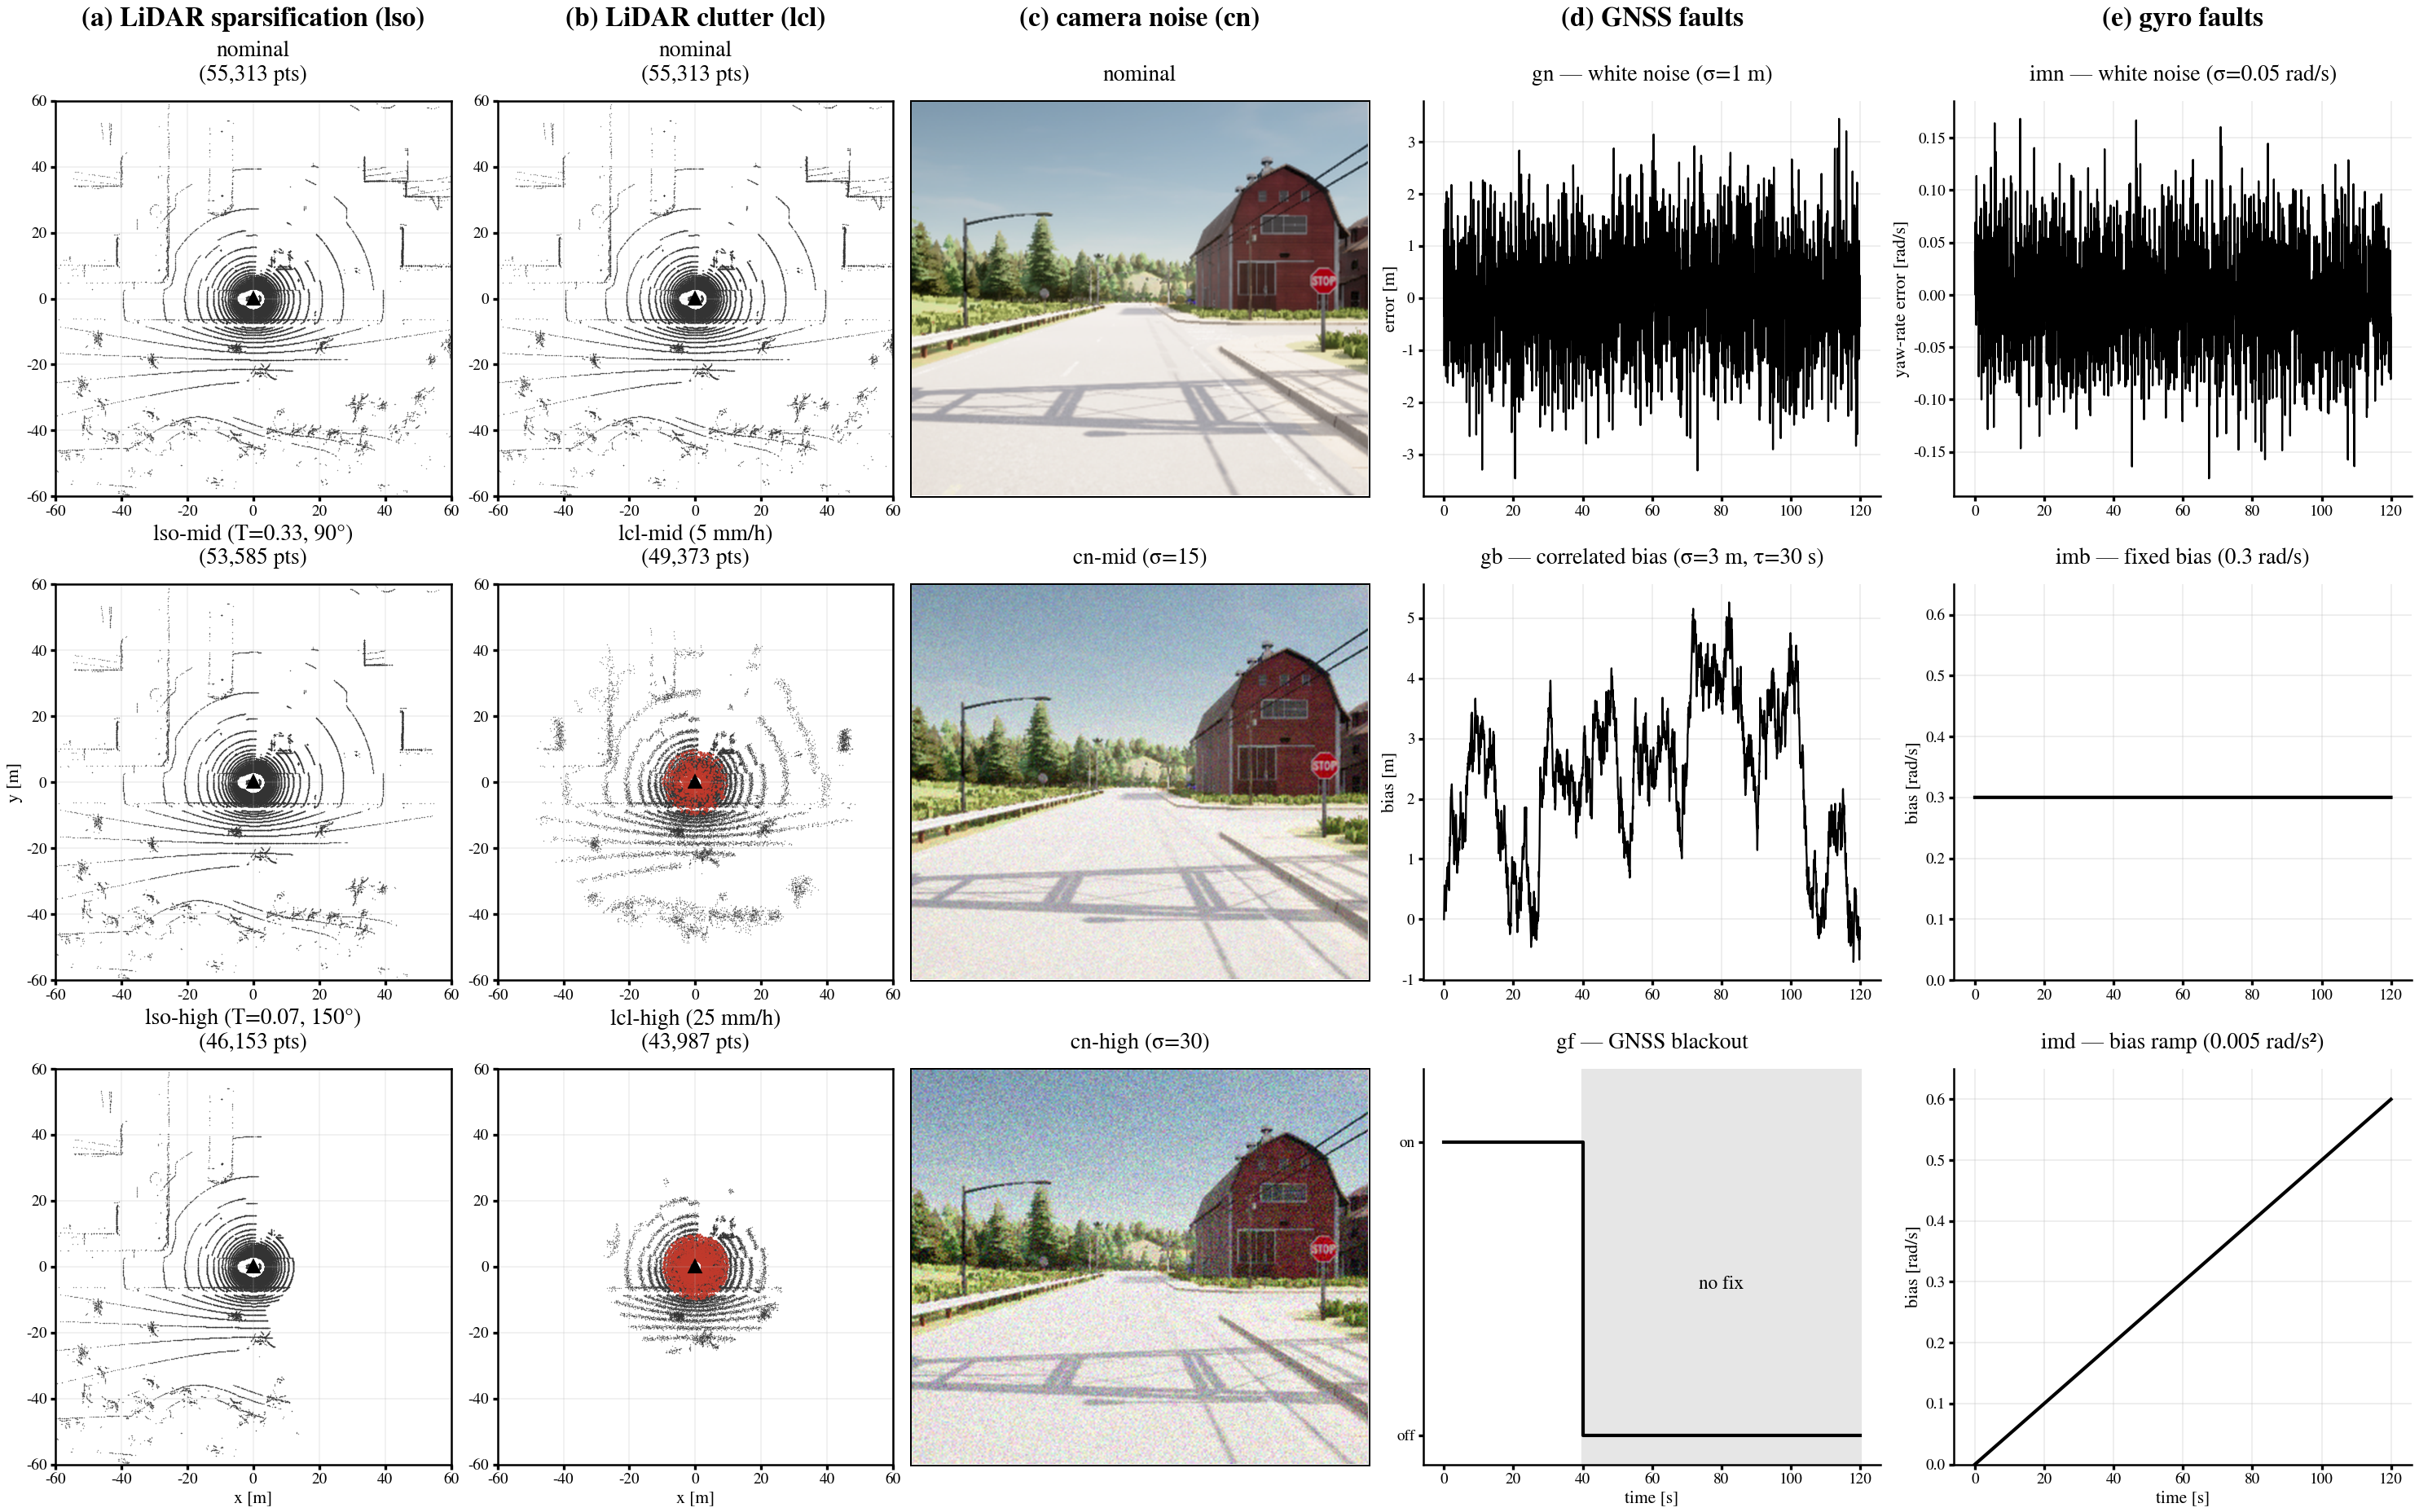
\includegraphics[width=0.82\textwidth]{figs/fig6_faults.png}
\caption{Sensor-level effects of fault injection---the injector's own
physics applied to one measured Town07 LiDAR scan and camera frame.
(a)~LiDAR sparsification (lso); (b)~LiDAR clutter (lcl, spurious returns
in red); (c)~camera pixel noise (cn); (d)~GNSS fault waveforms (gn/gb/gf);
(e)~gyro fault waveforms (imn/imb/imd). Panel parameters are the
injector's raw values for the severity definitions.}
\label{fig:faults}
\end{figure*}

\subsection{Collision Adjudication}
\label{sec:adjud}
The initial implementation adjudicated collisions with a collision
sensor attached to the pedestrian; measurement showed this sensor
\emph{never fired} in CARLA, and a listener death lost separation records,
so non-intervention-arm cases were being misjudged as avoided (affected
data were discarded and re-run). The reconstructed system has two layers:
(i)~\emph{primary}: a real-time ledger (RAW-HIT) written by the patched
callback of the ego's \texttt{sensor.other.collision} the moment a
collision occurs, with counterpart actor identifiers---unlike official
infraction tallies it survives early/forced termination; (ii)~\emph{audit}:
a pedestrian physics oracle (flung $>$4.5~m/s or a $>$5~m jump within
1~s) and the per-tick separation stream. Runner exit labels are refused as evidence (endpoint contacts,
post-collision stops, and infractions surviving only natural
termination). All encounter-level figures here are ledger-based; latencies use
simulation time.

\subsection{Encounter Experiments}
A decoupled injector process spawns pedestrian dart-outs at the right
lane edge with per-seed fixed walking speed, jitter, and fault waveform. Designs: (i)~a fault-free distance ladder at 4.2~m/s, spawn
distances $\{14,11,8,6,5\}$~m, $n{=}4$ each; (ii)~the same ladder blinded
(lso-high); (iii)~an 8~m encounter comparison under gn-mid (EKF input
contaminated, perception intact---so all arms share detection capability);
(iv)~a low-speed ladder at 3.0~m/s cruise; and (v)~a dose-response
experiment: caps $\{4.2,3.6,3.0\}$~m/s~$\times$ distances
$\{6,7,8,9\}$~m~$\times$ 10 seeds $=120$ runs, launched by a
\emph{settlement trigger}---the pedestrian spawns $D$~m ahead only when the
supervisor is in \texttt{MRM\_MOVE} and measured speed has stayed in the
cap-specific band for 1.0~s---so an encounter under an actually holding cap
is guaranteed at trigger level. The primary endpoint (8~m, paired 4.2 vs 3.0 exact McNemar) and a
manipulation-check adoption rule (first-tick speed in band $\pm$0.15~m/s,
ahead-of-ego geometry, launch within 420~s) were pre-specified; the sample
was fixed at 120 adopted runs.

\section{RESULTS}

\subsection{Detection Performance}
Table~\ref{tab:detect} summarizes the campaign: detection 96--100\% in
19 of 20 conditions---median latencies $\sim$1.0~s for hard fails
(simulation time), 2.1--8.6~s for degradation faults (wall clock)---with
zero false activations in 45 fault-free controls. The sole exception, mid-severity LiDAR sparsification (2\%), lies by
design in the tolerated band ($\sim$55~m effective range remains; the
supervisor deliberately continues driving); since tolerance cannot yet be
separated from channel insensitivity, we read the table as
\emph{intervention eligibility}. Notable structure: IMU-drift latency is inversely related to ramp slope
(8.6 vs 5.4~s)---small faults are caught later but become dangerous later;
GNSS-outage latency is bimodal (intended: a vehicle stopped at a red light
is not a risk exposure); and deferral stops split by family (GNSS
$\rightarrow$ comfortable, IMU $\rightarrow$ hard stops).

\begin{table}[t]
\caption{Detection rate and median latency per fault condition ($n{=}45$
unless noted; $\dagger$: navigation extension; *: simulation time, others
wall clock).}
\label{tab:detect}
\centering
\footnotesize
\setlength{\tabcolsep}{2pt}
\begin{tabular}{llcc}
\toprule
Fault & Sev. & Det.\ rate & Med.\ lat.\ (s) \\
\midrule
cf camera death & -- & 1.00 & 0.98* \\
cn camera noise & mid/high & 0.98/1.00 & 3.3/3.2 \\
lf LiDAR death & -- & 1.00 & 1.00* \\
lso LiDAR sparsif. & mid/high & 0.02/0.98 & --$^{c}$/5.0 \\
lcl LiDAR clutter & mid/high$^{a}$ & 1.00/0.96 & 4.8/4.5 \\
gn GNSS noise & mid/high & 1.00/1.00 & 2.1/4.4 \\
imn IMU noise & mid/high & 1.00/0.98 & 4.8/3.7 \\
gb$^{\dagger}$ GNSS corr.\ bias & mid/high & 1.00/1.00 & 3.0/2.3 \\
gf$^{\dagger}$ GNSS outage & -- & 1.00 & 3.2 (driving)$^{b}$ \\
imb$^{\dagger}$ IMU gyro bias & mid/high & 1.00/1.00 & 3.6/3.2 \\
imd$^{\dagger}$ IMU bias ramp & mid/high & 1.00/1.00 & 8.6/5.4 \\
\midrule
nf fault-free control & -- & \multicolumn{2}{c}{0 false activations / 45} \\
\bottomrule
\multicolumn{4}{l}{$^{a}$ lcl-high $n{=}26$ (final batch halted; accounted).}\\
\multicolumn{4}{l}{$^{b}$ bimodal: 21--40~s if the outage coincides with a stop.}\\
\multicolumn{4}{l}{$^{c}$ tolerated band; latency not reported.}
\end{tabular}
\vspace{-2mm}
\end{table}

Behind the binary rates lies the continuous signal
(Fig.~\ref{fig:health}): the decision variable
$\min(\mathrm{perception},\mathrm{cap_{loc}})$ separates into distinct
bands by fault intensity---fault-free runs never fell below 0.71 after
warm-up (consistent with zero false activations), mid severities stay in
the tolerated band, and high severities depart immediately on
injection---the basis of the graded normal/evacuate/defer structure.

\begin{figure}[t]
\centering
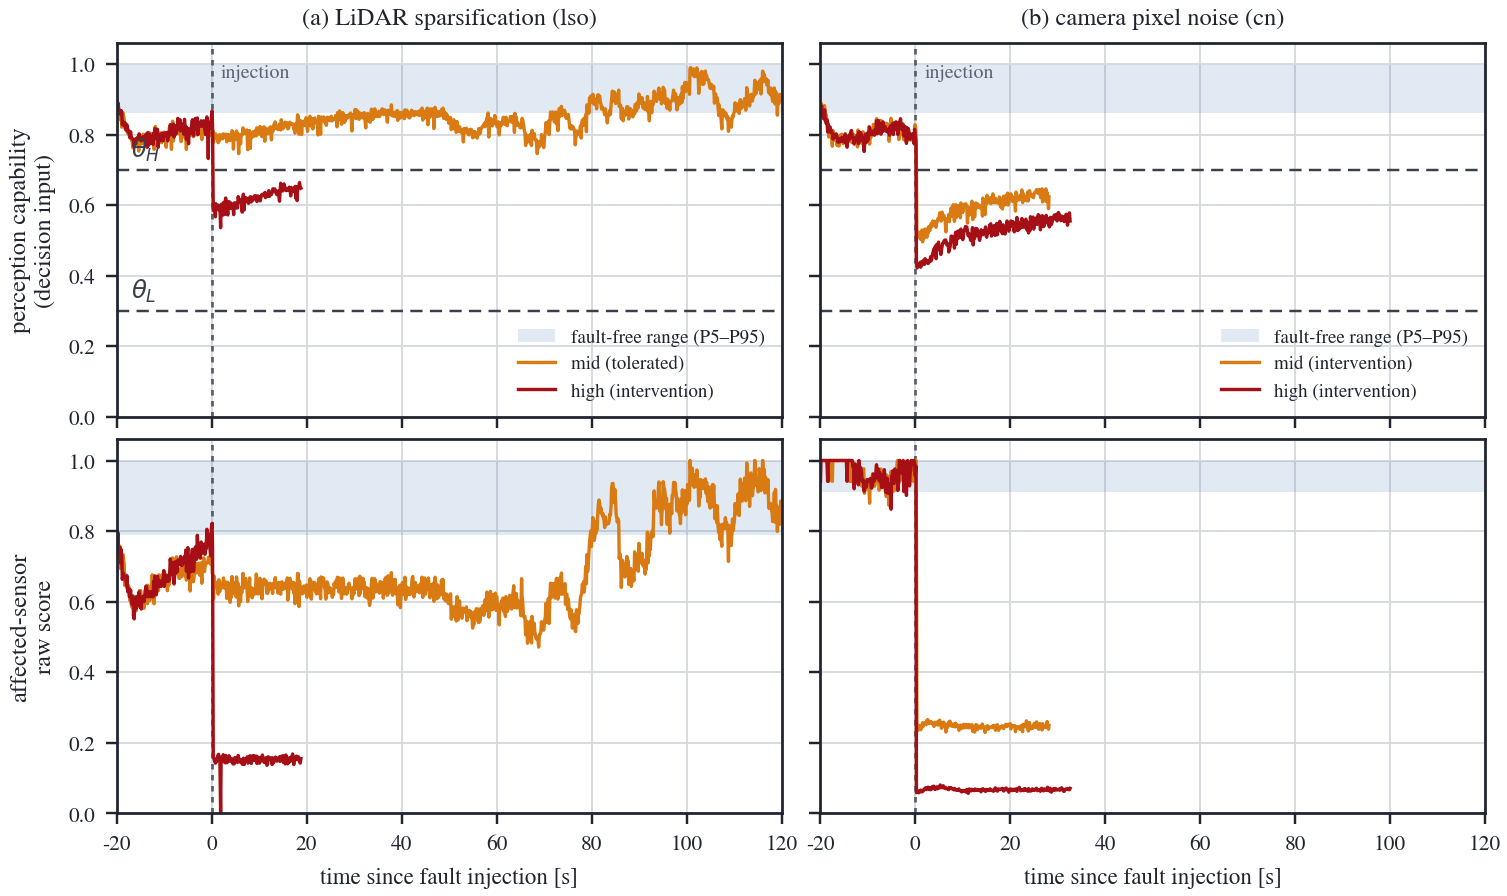
\includegraphics[width=0.94\columnwidth]{figs/fig12_health.png}
\caption{Injection-aligned health traces (top: the perception
capability score feeding the 0.7/0.3 transitions; bottom: raw sensor
score). Fault-free stays in the normal band, mid severity in the tolerated
band, high severity departs immediately---the band separation underlying
the graded response.}
\label{fig:health}
\end{figure}

\subsection{Graded Evacuation Behavior and Exposure}
For faults preserving the capability to move, the proposal evacuated
while the baseline (by definition) stopped in lane: camera death 16/45
shoulder evacuations (27 intended deferrals, 2 maneuver incompletions),
camera noise 25/90, GNSS noise 42/90. Severity mattered most in the
navigation family: gn-mid produced 40/45 evacuations while
gn-high converged to deferral in 42/45---movement is abandoned when
localization confidence falls below the movement minimum; conversely
lso-mid continued driving deliberately (response proportional to degree). Unmonitored (mrm-off, one run per type) the stack completed 238--275~m
faulted; with monitoring, exposure became a policy variable: 32--58~m for
detect+evacuate, 9--18~m for detect+stop (11--12~m for LiDAR clutter). The
stop minimizes exposure at the cost of lane occupancy; evacuation accepts
tens of meters of controlled exposure for lane clearance and an off-lane
refuge.

\subsection{Avoid/Collide Boundary and the 8~m Encounter}
The fault-free ladder at 4.2~m/s produced a clean staircase: 14 and 11~m
avoided 4/4 each; 8, 6, 5~m collided 4/4 each---boundary in 8--11~m,
matching Eq.~\eqref{eq:stop}'s 8.8~m (the same data calibrated the
model---self-consistency). Blinded (lso-high), the
stock stack froze mid-road before the encounter at 14/11~m and collided at
$\le$8~m: an unmonitored degraded vehicle either stands still or strikes.

Under gn-mid (perception intact, so all arms share detection
capability), an 8~m dart-out gave: stock at 4.2~m/s collided 10/10; the
proposed low-speed settled cruise avoided 8/8 and completed evacuation
(auxiliary Fisher $p=2.3\times10^{-5}$); and---critically---the
\emph{same} policy collided 2/2 in the deceleration transient
(3.5--3.8~m/s): protection begins only after deceleration completes. The
low-speed ladder placed the 3.0~m/s boundary at 7--8~m (8~m: 8/8 avoided;
7/6/5~m: 2/2 collisions each).

\subsection{Dose-Response Verification of the Speed Cap}
\label{sec:dose}
Because the two ladders used different launch protocols, the cap effect
was verified in a controlled pre-registered experiment on settled
encounters only, after fixing a cap-delivery interface defect (the earlier
``capped'' runs were receiving no cap---publish records are not delivery;
measured speed is). All 120 adopted runs passed the manipulation check
(per-arm first-tick speeds 4.05--4.13, 3.37--3.58, 2.60--3.07~m/s; five
failing runs re-run blind to outcome). Results (Table~\ref{tab:dose}) are monotone along both axes.
At the pre-specified primary endpoint (8~m), cap~4.2 collided in all ten
seeds and cap~3.0 in none---discordant pairs 10:0, exact McNemar two-sided
$p=0.002$: once the cap actually holds, its collision-reduction effect is
detected with unanimous seed-level directionality. The boundary moves
inward monotonically (Table~\ref{tab:dose}), corroborating the low-speed
ladder's 7--8~m interval. Interpretation limits: the causal conclusion is restricted to the
settled regime (the cap creates the post-settling margin, not transient
protection); no optimality is claimed for 3.0~m/s; cells are $n{=}10$,
single fault, single corridor.

\begin{table}[t]
\caption{Dose-response: collisions per cell ($n{=}10$ seeds, ledger
adjudication, settled encounters).}
\label{tab:dose}
\centering
\footnotesize
\setlength{\tabcolsep}{2pt}
\begin{tabular}{lccccl}
\toprule
Cap (m/s) & 6~m & 7~m & 8~m & 9~m & Boundary \\
\midrule
4.2 (control) & 10/10 & 10/10 & 10/10 & 10/10 & $>$9~m \\
3.6           & 10/10 & 10/10 & 10/10 & 2/10  & $\sim$9~m \\
3.0 (policy)  & 8/10  & 5/10  & 0/10  & 0/10  & $\sim$7~m \\
\bottomrule
\end{tabular}
\vspace{-2mm}
\end{table}

\subsection{Hard-Fail Decision Latency}
Hard fails are decided by an evidence-aware fast path (skipping
noise-oriented debounce and futile recovery holds) against an internal
1.5~s design deadline (not an FTTI-compliance claim). Over the full
camera/LiDAR-death matrices, ledger-based simulation-time latencies gave
medians $\approx$1.0~s, maximum 1.20~s, zero violations, with MRM
attainment maintained in full.

\section{DISCUSSION AND LIMITATIONS}

\textbf{Stop vs.\ evacuation is a temporal trade-off.} The in-lane stop
showed the lowest collision rate even under transient-window launches, at
the price of sustained lane occupancy; evacuation accepts controlled moving
exposure and residual transient risk but on success clears the lane to an
off-lane refuge. Neither is unconditionally superior; the choice should follow the
fault's temporal structure---concrete selection variables for
ISO~23793-1.

\textbf{Residual risk is temporally localized.} All evacuation-arm
collisions occurred before deceleration completed (transient 2/2), none
after settling (0/8). Distinguishing the post-detection transient from the overall
fault-response risk window ($T_{\mathrm{detect}}+T_{\mathrm{decel}}$), the
results support---observationally, not causally---that earlier detection
and faster deceleration shrink this window, widening the FTTI margin.

\textbf{Adjudication lessons generalize.} ``Zero collisions'' is
meaningful only after the verdict channel is proven alive:
positive-control checks of collision sensors, physics-oracle cross-checks,
and refusal to read absence of a record as absence of an event. The
silently undelivered cap carries the same lesson---actuation must be
verified by downstream effect; the real-time ledger was the remedy.

\textbf{Limitations.} Single map, single 15~km/h limit, two launch
corridors: the numeric boundaries and dose-response values are
low-speed-ODD numbers; generalizable claims are structural (boundary's
stopping-distance dependence, transient risk concentration, the
stop/evacuation trade-off). Autoware observations are version-specific
(0.39.0). Dose-response cells are $n{=}10$ with wide CIs; testing was
restricted to the pre-specified endpoint. Campaign-level collision-free
status predates the ledger (no pedestrian injections there). The dynamic
detection budget was not ablated against a fixed deadline;
hazard-time-referenced compliance needs an instrumentation extension; the
health-proportional cap is implemented but unevaluated; no real-vehicle
validation.

\section{CONCLUSION}

We proposed and validated, in an Autoware--CARLA closed loop of 1{,}862
valid cases, a supervisory add-on layer estimating sensor faults as
continuous health scores and selecting MRMs in a graded manner, with a
conservative cap on evacuation movement. Three conclusions carry beyond
the numbers. First, shoulder evacuation is no panacea: stopping and evacuation form
a temporal trade-off between immediate collision risk and lane clearance,
and the choice should follow the fault's temporal structure. Second,
evacuation's residual risk concentrates in the post-detection transient,
while settled low speed verifiably moves the boundary inward (transient
2/2 vs.\ settled 0/8; dose-response 10:0, $p=0.002$)---supporting earlier
detection and faster deceleration within the FTTI. Third, simulation safety claims hold only
on a validated adjudication framework; the ledger/physics-oracle scheme
and catalogued pitfalls are reusable for any simulated MRM comparison. Future work: high-speed ODDs and maps, formalizing the detection
budget, the health-proportional cap, and real-vehicle validation.

\begin{thebibliography}{99}
\footnotesize
\bibitem{iso26262} ISO 26262:2018, \emph{Road vehicles --- Functional safety}.
\bibitem{iso21448} ISO 21448:2022, \emph{Road vehicles --- Safety of the intended functionality}.
\bibitem{j3016} SAE J3016\_202104, \emph{Taxonomy and Definitions for Terms Related to Driving Automation Systems}, 2021.
\bibitem{iso23793} ISO 23793-1:2024, \emph{Intelligent transport systems --- Minimal risk manoeuvre (MRM) for automated driving --- Part 1}.
\bibitem{iso3691} ISO 3691-4:2023, \emph{Industrial trucks --- Safety requirements --- Part 4: Driverless industrial trucks}.
\bibitem{isermann} R. Isermann, ``Model-based fault-detection and diagnosis --- status and applications,'' \emph{Annu.\ Rev.\ Control}, vol.~29, no.~1, 2005.
\bibitem{autoware} Autoware Foundation, ``autoware.universe documentation'' (evaluated version 0.39.0), autowarefoundation.github.io/autoware.universe.
\bibitem{trierweiler} M. Trierweiler \emph{et al.}, ``Influence of sensor blockage on automotive LiDAR systems,'' in \emph{Proc.\ IEEE SENSORS}, 2019.
\bibitem{goodin} C. Goodin \emph{et al.}, ``Predicting the influence of rain on LIDAR in ADAS,'' \emph{Electronics}, vol.~8, no.~1, 2019.
\bibitem{langel} S. Langel, O. Garc\'ia Crespillo, and M. Joerger, ``Overbounding the effect of uncertain Gauss-Markov noise in Kalman filtering,'' \emph{NAVIGATION}, vol.~68, no.~2, 2021.
\bibitem{pek} C. Pek \emph{et al.}, ``Using online verification to prevent autonomous vehicles from causing accidents,'' \emph{Nat.\ Mach.\ Intell.}, vol.~2, 2020.
\bibitem{reschka2015safe} A. Reschka and M. Maurer, ``Conditions for a safe state of automated road vehicles,'' \emph{it --- Inf.\ Technol.}, vol.~57, no.~4, 2015.
\bibitem{xue2018} W. Xue \emph{et al.}, ``A fallback approach for an automated vehicle encountering sensor failure in monitoring environment,'' in \emph{Proc.\ IEEE IV}, 2018.
\bibitem{tang} J. Tang, C. Yang, and H. Nishimura, ``Minimum risk maneuver strategy for automated driving system under multiple conditions of sensor failure,'' \emph{Systems}, vol.~14, no.~1, 2026.
\bibitem{reschka2015ability} A. Reschka \emph{et al.}, ``Ability and skill graphs for system modeling, online monitoring, and decision support for vehicle guidance systems,'' in \emph{Proc.\ IEEE IV}, 2015.
\bibitem{carla} A. Dosovitskiy \emph{et al.}, ``CARLA: An open urban driving simulator,'' in \emph{Proc.\ CoRL}, 2017.
\bibitem{awcl} G. Kaljavesi, D. Majstorovic, M. Clement, and F. Diermeyer, autoware\_carla\_leaderboard (Autoware--CARLA leaderboard coupling), TUM Institute of Automotive Technology, preprint, 2026.
\end{thebibliography}

\end{document}
